\chapter{Sistemas de numeração}
\label{sinais}

Os sistemas de numeração são diferentes formas para representação de quantidades. Esta representação é feita organizando os dígitos em função de uma determinada base. 

Também é importante entender que um sistema poderá ser aplicável em algumas siutações e em outras não. A seguir alguns dos principais sistemas de numeração conhecidos:

\begin{itemize}
	\item Sistema Unário: Remonta a idade antiga na históira da humanidade. A contagem era feita pelo método da comparação. O pastor, ao contar suas ovelhas, precisava de uma bolsa contendo uma pedra pra cada ovelha. 
	\item Sistema Duodecimal: Deu origem aos termos dúzia e grosa\footnote{1 dúzia de dúzias.}. Este sistema não é muito difundido e acredita-se que tenha surgido com a contagem das falanges dos dedos para contar. 
	\item Sistema Sexagesimal: Deu origem ao sistema de contagem de horas, minutos e segundos, bem como ângulos em graus.
\end{itemize}

Atualmente o princpal sistema numérico é o decimal, revisado na seção~\ref{sistemaDecimal}. Em Ciência da Computação os sistemas mais usados são o binário, o hexadecimal e o octal, discutidos na seção~\ref{basesComput}.

\section{Revisão do sistema Decimal}
\label{sistemaDecimal}

Quanto estávamos no ensiono fundamental, alguns de nossos professores nos ensinaram a ler um número usando uma ferramenta concreta chamada Quadro Valor de Lugar. Neste quadro, apresentado na Figura~\ref{fig:qvl}, os professores ensinaram que quando colocamos um numero ali ele tem um valor em funçao da posição que ocupa. 

\begin{figure}[h]
	\begin{center}
		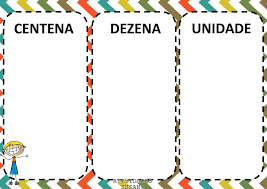
\includegraphics[width=0.6\textwidth]{img/sistemasNum/qvl.png}
		\caption{Quadro Valor de Lugar (Fonte: Figura da Internet)}
		\label{fig:qvl}
	\end{center}
\end{figure}

Descrição da Figura~\ref{fig:qvl}: Uma diagrama com 3 espaços vazios identificados como Unidade, Dezena e Centena, nessa ordem da direita para esquerda. O diagrama possui motivos infantis e marcações coloridas.

Por exemplo: ao preencher o quadro com os números 1 (na centena), 2 (na dezena) e 4 (na unidade), o valor encontrado será \(100 + 20 + 4\), ou seja Cento e Vinte e Quatro.

Isto acontece porque o sistema decimal é posicional, ou seja, o dígito assume um valor em função de sua posição na representação numérica. Isto pode ser explicado matematicamente pelo polinômio da Fórmula~\ref{polinomio}, que demonstra:

\begin{equation}\label{polinomio}
N=d_1.\beta^{1-1}+d_2.\beta^{2-1}+d_3.\beta^{3-1}+d_4.\beta^{4-1}+...d_t.\beta^{t-1}
\end{equation}

onde,
\begin{itemize}
	\item N: Valor do número;
	\item $\beta$: Base do número;
	\item t: Tamanho do número ou quantidade de dígitos (iniciando em 1);
	\item $d_t$: Dígito na posição;
\end{itemize}

Esta equação pode representada de forma mais condensada, fazendo uso da simbologia de somatório\footnote{"Google it".}. Veja a Equação~\ref{eq:sum}

\begin{equation}\label{eq:sum}
N=\sum_{i=1}^{t}d_i.\beta^{i-1}
\end{equation}

Para melhor compreensão vamos resolver o caso anteriormente resolvido pelo Quadro Valor de Lugar. Usamos uma tabela para melhor representar a ideia.

\noindent\textbf{Exemplo: 124}
\begin{table}[h]
	\centering
	\begin{tabular}{|c|r|r|r|r|}
		\hline
		Dígitos 	&  & 1 & 2 & 4  \\
		\hline
		Posição do dígito na representação:	& 4 & 3 & 2 & 1  \\
		\hline
	\end{tabular}
\end{table}

Observe que não há um numero na posição 4 - seria uma 'casa vazia'.

Sabendo que a base é decimal, portanto $\beta=10$ e aplicando a equação~\ref{eq:sum} temos:

\begin{center}
\( N=4.10^{0}+2.10^{1}+1.10^{2}\) \\
\( N=4.1+2.10+1.100 \) \\
\( N=4+20+100 \) \\
\( N = 124\)\\
\end{center}
Ou seja, a representação 124 tem valor Cento e Vinte e Quatro. 


\section{Bases numéricas da Computação}
\label{basesComput}
O sistema posicional apresentado no cálculo do valor da representação numérica é o mesmo para os outros sistemas, mudando apenas a base.

\subsection{Binária}
\subsection{Hexadecimal}
\subsection{Octal}

\section{Introdução à aritmética binária}
\label{aritmetica}

Segundo definição do dicionário Oxford, aritmética é a parte da matemática que estuda (ou, por assim dizer, trabalha) com as operações numéricas de soma, subtração, multiplicação, divisão, entre outras.

Nesta sessão iremos discutir o básico sobre operações aritméticas soma e substração na base binária.

\subsection{Soma binária}
\label{somabinaria}

A soma de números binários é muito semelhante a soma de números decimais. O método é exatamente o mesmo, mudando apenas a base utilizada.

Os valores das somas são:
\begin{itemize}
	\item 0 + 1 = 1
	\item 1 + 0 = 1
	\item 1 + 1 = 10
	\item 1 + 1 + 1 = 11
\end{itemize}

No caso de operações com números binários com mais que um dígito é preciso sempre somar os dígitos correspondentes enter os números da conta.

Em binário, sempre que o resultado da soma der um número maior que 1 a resposta vai ocupar 2 dígitos. Veja a soma a seguir:
\begin{itemize}
	\item 1 + 1 = 10
\end{itemize}
Onde a resposta é 10 (que tem dois dígitos). Neste caso é preciso separar o número 10 em duas partes. 
A parte menos significativa (digito mais a direita) fica nesta parte da resposta enquanto que a parte mais significativa (digito mais a esquerda) vai para a próxima casa. O que chamamos normalmente de vai-um.

O mesmo ocorre na soma a seguir:
\begin{itemize}
	\item 1 + 1 +1 = 11
\end{itemize}
Onde a resposta é 11. Neste caso fica 1 e vai 1 para a próxima casa.


\textbf{Exemplo A):}
\begin{equation}\label{eq1}
101 + 10
\end{equation}

Armando a conta:
\begin{table}[h]
\centering
	\begin{tabular}{r|rrr}
		 	dígitos	& $d_2$ & $d_1$ & $d_0$ \\
		1ª parcela  & 1 & 0 & 1 \\
		2ª parcela  &   & 1 & 0 \\
		\hline
		   soma	  & 1 & 1 & 1 \\
	\end{tabular}
\end{table}

De forma descritiva:

No exemplo da equação~\ref{eq1}, iniciamos somando os dígitos menos significativos ($d_0$) dos dois números, que no caso são $ 1 + 0 = 1$. A resposta desta parcial é 1, sem "vai-um".

A seguir, indo da direita para esquerda, somamos os números do próximo digito ($d_1$), no caso $ 0 + 1 = 1$. A resposta desta parcial é 1, sem "vai-um".

Por fim, somamos os números do próximo dígito ($d_2$), que no caso é apenas $1$, pois o segundo número não possui valor neste dígito. A resposta desta parcial é 1, sem "vai-um".

A resposta final da operação é 111.

Podemos verificar a operação simplesmente convertendo tudo para decimal. Convertendo 101 para decimal temos 5 e convertendo 10 para decimal tempos 2. 

E 5+2=7, onde 7 = 111 em binário.


\textbf{Exemplo B):}
\begin{equation}\label{eq2}
101 + 11
\end{equation}

Armando a conta:
\begin{table}[h]
	\centering
	\begin{tabular}{r|rrrr}
		"vai-um"	&  	1	&  	1	& 1		& 		\\
		dígitos		& $d_3$	& $d_2$ & $d_1$ & $d_0$ \\
		1ª parcela  &  		&   1 	& 0 	& 1 \\
		2ª parcela  &  		&   	& 1 	& 1 \\
		\hline
		soma	  	&  	1	&   0 	& 0 	& 0 \\
	\end{tabular}
\end{table}

De forma descritiva:

No exemplo da equação~\ref{eq2}, iniciamos somando os dígitos menos significativos ($d_0$) dos dois números, que no caso são $ 1 + 1 = 10$. A resposta dessa parcial é 0 e "vai-um", ou seja, na casa do $d_0$ fica o dígito 0 e o 1 vai para a próxima, no caso $d_1$. 

Indo para a esquerda, vamos executar a conta dos dígitos na casa $d_1$, que no caso são $1 + 0 + 1 = 10$. A resposta dessa parcial é 0 e "vai-um", ou seja, na casa do $d_1$ fica o dígito 0 e o 1 vai para a próxima ($d_2$).

Seguindo mais para a esquerda, passamos para a casa $d_2$, que no caso deverá executar $1 + 1 = 10$. A reposta dessa parcial é 0 e "vai-um", ou seja, na casa $d_2$ fica o dígito 0 e o 1 vai para próxima ($d_3$).

Na casa $d_3$ temos apenas o dígito que veio da operação anterior e não soma com nada - o resultado dessa parcial é 1.

No final temos o número $1000$.


\subsection{Subtração binária}

A subtração em binário segue a mesma lógica sa subtração no sistema decimal. 

Os valores das subtrações são:
\begin{itemize}
	\item 0 - 0 = 0
	\item 1 - 1 = 0
	\item 1 - 0 = 1
	\item 0 - 1 = -1
	\item 10 - 1 = 1
\end{itemize}

Caso o número tenha mais dígitos. Se um dígito do subtraendo for menor que dígito correspondente do minuendo será necessário "pedir emprestado".

\textbf{Exemplo A):}
\begin{equation}\label{eq3}
111 - 10 = 110
\end{equation}

Armando a conta:
\begin{table}[h]
	\centering
	\begin{tabular}{r|rrrr}
		dígitos		& $d_3$	& $d_2$ & $d_1$ & $d_0$ \\
		subtraendo  &  		&   1 	& 1 	& 1 \\
		minuendo 	&  		&   	& 1 	& 0 \\
		\hline
		diferença  	&  		&   1 	& 0 	& 1 \\
	\end{tabular}
\end{table}

De forma descritiva: 
Tal como a soma, a subtração é iniciada pelos dígitos menos significativos, (direita para esquerda). No exemplo da equação~\ref{eq3}, caso o dígito $d_0$ subtraímos 0 de 1, onde o resultado é 1.

Indo para esquerda, no dígito $d_1$, subtraímos 1 de 1, onde o resultado é 0.

Agora no dígito $d_2$ subtraímos nada (poderíamos dizer 0) de 1, resultado em 1.

A resposta final é 101.

\textbf{Exemplo B):}
\begin{equation}\label{eq4}
110 - 1 = 101
\end{equation}

Armando a conta:
\begin{table}[h]
	\centering
	\begin{tabular}{r|rrrr}
		dígitos		& $d_3$	& $d_2$ & $d_1$ & $d_0$ \\
		subtraendo  &  		&   1 	& 1 	& 0 \\
		minuendo 	&  		&   	& 	 	& 1 \\
		\hline
		diferença  	&  		&   1 	& 0 	& 1 \\
	\end{tabular}
\end{table}

De forma descritiva: 

No exemplo da equação~\ref{eq4}, iniciamos pelo dígito menos significativo ($d_0$), onde subtraímos 1 de 0. Esta operação daria um resultado negativo, mas como o subtraendo é maior que o minuendo, podemos "pegar emprestado" do próximo dígito. Desta forma o dígito $d_2$ empresta uma unidade para o dígito $d_0$. Quando este dígito troca de posição (salta de uma posição maior para uma menor), passa para a posição menor tendo o valor da base. Em outras palavras, emprestamos 1, mas ao chegar na casa do $d_0$ veio valendo 10. Agora poderemos subtrair 1 de 10, operação que tem como resposta 1.

O digito $d_1$ que antes era 1 agora é 0 (isso porque "emprestou 1"). Ao subtrairmos 0 de 0 temos resultado 0.

Na posição do dígito $d_2$ subtraímos 0 de 1, tendo o resultado 1.

O resultado final da operação é 101.

\textbf{Exemplo C):}
\begin{equation}\label{eq5}
1001 - 11 = 1
\end{equation}

Armando a conta:
\begin{table}[h]
	\centering
	\begin{tabular}{r|rrrr}
		dígitos		& $d_3$	& $d_2$ & $d_1$ & $d_0$ \\
		subtraendo  &  	1	&   0 	&   0 	& 1 \\
		minuendo 	&  		&   	& 	1 	& 1 \\
		\hline
		diferença  	&  		&   1 	&   1 	& 0 \\
	\end{tabular}
\end{table}

De forma descritiva: 

No exemplo da equação~\ref{eq5}, iniciamos a operação no dígito $d_0$, subtraindo 1 de 1, resultando em 0.

No dígito $d_1$, precisamos subtrair 1 de 0, sendo necessário pegar "emprestado" de $d_2$. Ao fazer isso, passamos a subtrair 1 de 10, resultado em 1.

O dígito $d_2$ agora vale -1, porque emprestou 1 "sem ter para emprestar". Nessa posição precisamos subtrair 0 de -1 e para isso vamos pedir emprestado de $d_3$. Ao fazer isso, o valor dessa casa fica 1 (porque $10 - 1 = 1 $). Então o resultado dessa posição será 1.

Na casa $d_3$, que "emprestou" 1, ficamos agora com 0, que subtraído de 0 dá 0.

O resultado final da operação é 110.


\section{Representação de números negativos}
\label{numerosNegativos}

Em sistemas digitais e na computação como um todo, os únicos símbolos que temos para trabalhar são o \emph{0} e o \emph{1}. Todos os outros símbolos precisam ser construídos a partir destes. 

Esta regra se aplica também aos símbolos de números negativos. Como, digitalmente, dizemos para um computador que um número é negativo? como o número negativo é armazenado na memória de um computador? Nesta seção vamos demonstrar 2 métodos (técnicas) conhecidos.

Note quem em todas as técnicas temos apenas uma quantidade definida de bits, com 0 ou 1. A utilização das técnicas varia conforme a aplicação.

Todos os exemplos vão trabalhar com \emph{6 bits}. Em uma máquina real esta quantidade de bits será compatível com a arquitetura da máquina e a técnica adotada poderá ser uma variação das aqui apresentadas.

\subsection{Sinal-Magnitude}
\label{sinalMagnitude}
Neste técnica reservamos o bit mais significativo para representar o sinal e o restante dos bits são usados para representar o valor do número (magnitude).

Com 6 bits o maior número que conseguiremos representar será +31, e o menor número será -31. Isto porque o sexto bit é reservado para o sinal.

\noindent\textbf{Número  -10}

Para representar o número -10, o bit mais a esquerda (o mais significativo) fica 1, pois está reservado para o sinal. Os outros 5 bits são usados para o número ficando 01010.

\begin{table}[h]
	\centering
	\begin{tabular}{|r|r|r|r|r|r|}
		\hline
		1 & 0 & 1  & 0 &  1 & 0 \\
		\hline
	\end{tabular}
\end{table}


\noindent\textbf{Representar +15}

Para representar o número +15, o bit mais a esquerda (o mais significativo) fica 0, pois está reservado para o sinal. Os outros 5 bits são usados para o número ficando 01111.

\begin{table}[h]
	\centering
	\begin{tabular}{|r|r|r|r|r|r|}
		\hline
		0 & 0 & 1  & 1 &  1 & 1 \\
		\hline
	\end{tabular}
\end{table}

\noindent\textbf{Representar -27}

Para representar o número -27, o bit mais a esquerda (o mais significativo) fica 1, pois está reservado para o sinal. Os outros 5 bits são usados para o número ficando 11011.

\begin{table}[h]
	\centering
	\begin{tabular}{|r|r|r|r|r|r|}
		\hline
		1 & 1 & 1  & 0 &  1 & 1 \\
		\hline
	\end{tabular}
\end{table}

\subsection{Complemento de 1}
\label{compl1}
O Complemento de 1 consiste em inverter os bits do número um-a-um. 

\noindent\textbf{Representar -10}
\begin{table}[h]
	\centering
	\begin{tabular}{|l|r|r|r|r|r|r|}
		\hline
		10 em binário: 		& 0 & 0 & 1  & 0 &  1 & 0 \\
		\hline
		Complemento de 1: 	& 1 & 1 & 0  & 1 &  0 & 1 \\
		\hline
	\end{tabular}
\end{table}

Este procedimento é base para o Complemento de 2, descrito na seção~\ref{compl2}. 

\subsection{Complemento de 2}
\label{compl2}
O Complemento de 2 é uma técnica que consiste aplicar o Complemento de 1 e somar 1 no fim - o resultado deste procedimento representa o número negativo. 

É sempre necessário ter um bit a mais para fazer a representação, ou seja, se o número precisa de 5 bits para representar seu valor, será necessário mais 1 para o complemento.

Dentre todas, esta técnica é mais utilizada, pois podemos fazer operações aritméticas diretamente com o número em Complemento de 2. 

\noindent\textbf{Representar -10}

10 em binário é 1010, com 6 bits temos 00 1010. Os passos para passar esse número para Complemento de 2 são:

\begin{table}[h]
	\centering
	\begin{tabular}{|r|r|r|r|r|r|r|}
		\hline
		10 em binário: 			& 0 & 0 & 1  & 0 &  1 & 0 \\
		\hline
		Complemento de 1: 		& 1 & 1 & 0 & 1 & 0 & 1 \\
		\hline
		Soma 1 					&  	&  	&  	&	&	& 1 \\
		\hline
		\hline
		-10 em Complemento de 2:	& 1 & 1 & 0	& 1 & 1 & 0 \\
		\hline
	\end{tabular}
\end{table}
O número 11 0110 é -10 na notação Complemento de 2.

\noindent\textbf{Representar -23}

23 em binário é 1 0111, com 6 bits temos 01 0111. 
\begin{table}[h]
	\centering
	\begin{tabular}{|r|r|r|r|r|r|r|}
		\hline
		23 em binário: 			& 0 & 1 & 0  & 1 & 1 & 1 \\
		\hline
		Complemento de 1: 		& 1 & 0 & 1  & 0 & 0 & 0 \\
		\hline
		Soma 1 					&  	&  	&  	&	&	 & 1 \\
		\hline
		\hline
		-23 em Complemento de 2:	& 1 & 0 & 1	& 0 & 0 & 1 \\
		\hline
	\end{tabular}
\end{table}


\section{Operações aritméticas em Complemento de 2}
\label{aritmeticaCompl2}

Uma das vantagens da notação Complemento de 2(seção~\ref{compl2} é que ela possibilita o uso de operações aritméticas. A operação é sempre soma (não precisa fazer subtração) e se o resultado for negativo a resposta ja sai em Complemento de 2.

Vamos demonstrar isso por meio de 4 exemplos, todos com 6 bits.

\subsection{Somar Positivo com Positivo}
Neste caso os números não estão em complemento de 2 e soma acontece diretamente.

\noindent\textbf{Exemplo: 10 + 5}
\begin{table}[h]
	\centering
	\begin{tabular}{|r|r|r|r|r|r|r|}
		\hline
		10 em binário: 	& 0 & 0 & 1  & 0 & 1 & 0 \\
		\hline
		5 em binário:	& 0 & 0 & 0  & 1 & 0 & 1 \\
		\hline
		\hline
		Resultado (15):		& 0	& 0 & 1  &1	 & 1 & 1 \\
		\hline
	\end{tabular}
\end{table}


\subsection{Somar Positivo MAIOR com Negativo MENOR}

\noindent\textbf{Exemplo: 10 + -5}

O operando que for negativo, no caso -5, precisa ser convertido para a Notação Complemento de 2. 

A resposta esperada é um número positivo (+5). Ao efetuarmos a conta veremos que o resultado já está no formato certo.


\begin{table}[h]
	\centering
	\begin{tabular}{|r|r|r|r|r|r|r|r|}
		\hline
						& $d_6$ & $d_5$ & $d_4$ & $d_3$  & $d_2$ & $d_1$ & $d_0$ \\
		\hline
		10 em binário: 	&	& 0 & 0 & 1  & 0 & 1 & 0 \\
		\hline
		-5 em binário:	&	& 1 & 1 & 1  & 0 & 1 & 1 \\
		\hline
		\hline
		Resultado (+5):	& \textit{1*}  & 0	& 0 & 0  & 1 & 0 & 1 \\
		\hline
	\end{tabular}
\end{table}
* o 7º bit ($d_6$) excede a quantidade de bits "reservada" para a conta (que no caso é 6 bits). Neste caso este bit que excede é DESCARTADO. O bit mais significativo da reposta ($d_5$) tem valor 0, o que indica que o resultado é um número positivo.


\subsection{Somar Positivo MENOR com Negativo MAIOR}

\noindent\textbf{Exemplo: 4 + -7}

O operando que for negativo, no caso -7, precisa ser convertido para a Notação Complemento de 2. 

A resposta esperada é um número negativo (-3). Ao efetuarmos a conta veremos que o resultado já está no formato certo. -3 em Complemento de 2 com 6 bits é 111101.

\begin{table}[h]
	\centering
	\begin{tabular}{|r|r|r|r|r|r|r|r|}
		\hline			& $d_6$ & $d_5$ & $d_4$ & $d_3$  & $d_2$ & $d_1$ & $d_0$ \\
		\hline
		4 em binário: 	&	& 0 & 0 & 0  & 1 & 0 & 0 \\
		\hline
		-7 em binário:	&	& 1 & 1 & 1  & 0 & 0 & 1 \\
		\hline
		\hline
		Resultado (-3):	&   & 1	& 1 & 1  & 1 & 0 & 1 \\
		\hline
	\end{tabular}
\end{table}


\subsection{Somar Negativo com Negativo}

\noindent\textbf{Exemplo: -4 + -7}

Os operandos negativos, no caso -7 e -4, precisam ser convertidos para a Notação Complemento de 2. 

A resposta esperada também será um número negativo (-11). Ao efetuarmos a conta veremos que o resultado já está no formato certo. -11 em Complemento de 2 com 6 bits é 111101.

\begin{table}[h]
	\centering
	\begin{tabular}{|r|r|r|r|r|r|r|r|}
		\hline			& $d_6$ & $d_5$ & $d_4$ & $d_3$  & $d_2$ & $d_1$ & $d_0$ \\
		\hline
		-4 em binário: 	&	& 1 & 1 & 1  & 1 & 0 & 0 \\
		\hline
		-7 em binário:	&	& 1 & 1 & 1  & 0 & 0 & 1 \\
		\hline
		\hline
		Resultado (-11):	&\emph{1*} 	& 1 & 1 & 0  & 1 & 0 & 1 \\
		\hline
	\end{tabular}
\end{table}
* o 7º bit ($d_6$) excede a quantidade de bits "reservada" para a conta (que no caso é 6 bits). Neste caso este bit que excede é DESCARTADO. O bit mais significativo da reposta ($d_5$) tem valor 1, o que indica que o resultado é um número negativo.



bibliografia desta seção
3 História da matemática: e-book - como surgiram
alguns conceitos matemáticos? / Valdirene da Rosa
Rocho; Carla Margarete Ferreira dos Santos;
Margarete Faria Medeiros; Carla Sofia Dias Brasil;
Taís Pereira da Silva (Orgs.). -- Sombrio:
%Instituto Federal Catarinense, 2018. Disponível em %https://editora.ifc.edu.br/wp-content/uploads/sites/33/2018/11/e-book_historia_da_matematica_ultima_versao.pdf

FRAGA, Carina Ribeiro et al. Números naturais: introdução, sistemas de numeração. 2013.
http://www.labeduc.fe.usp.br/wp-content/uploads/Unidade-did%C3%A1tica-N%C3%BAmeros-Naturais-1.pdf